\subsection{Chapter 19 - Electric circuits}

\subsubsection{Overview}\label{chapter:circuits}

In this chapter, we develop the tools to model electric circuits. This will allow us to determine the current and voltages across different components, such as resistors and capacitors, within a circuit. We will also discuss how a battery can provide a current at a fixed potential difference, and how one can construct devices to measure current and voltages.

\begin{framed}
\textbf{Learning Objectives}\\
\begin{itemize}
\item Understand how a battery works.
\item Understand Kirchhoff's rules and how to apply them.
\item Understand how to model a circuit with resistors and/or capacitors.
\item Understand how an ammeter and voltmeter function, and how to model them.
\end{itemize}
\end{framed}

\begin{framed}
\textbf{Think About It}\\
If two outlets in your house are connected to the same circuit, are the outlets connected in series or in parallel?

\begin{enumerate}
\item series
\item parallel
\end{enumerate}

\begin{framed}
\textbf{Answer}\\
\begin{enumerate}[resume]
\item
\end{enumerate}
\end{framed}
\end{framed}

\subsubsection{Batteries and simple circuits}

:label: sec:circuits:batteries
A battery is an electric component that provides a constant electric potential difference (a fixed voltage) across its terminals. Luigi Galvani was the first to realize that certain combinations of metals placed into contact with each other can lead to an electric potential difference (or rather, he realized that they can make the legs of a dead frog twitch, which we now understand to be from the potential difference due to the metals). Effectively, Galvani created the first ``electrochemical cell''. Alessandro Volta then combined several of these cells together to form the ``voltaic pile'', which is what we would now call a battery (a battery is technically a combination of several cells, or a ``battery of cells'', although one often uses the term battery even if only a single electric cell is involved).

\paragraph{The electrochemical cell}

An electric cell can be constructed from metals that have different affinities to be dissolved in acid. A simple cell, similar to that originally made by Volta, is comprised of two metal electrodes placed in a liquid called electrolyte, as illustrated in Figure~\ref{fig:circuits:electriccell}. Common materials used are carbon (Volta used silver) and zinc for the electrodes, and sulfuric acid for the electrolyte. Before the cell is constructed, the electrodes and the electrolyte are all electrically neutral.

\begin{figure}[!htbp]
\centering
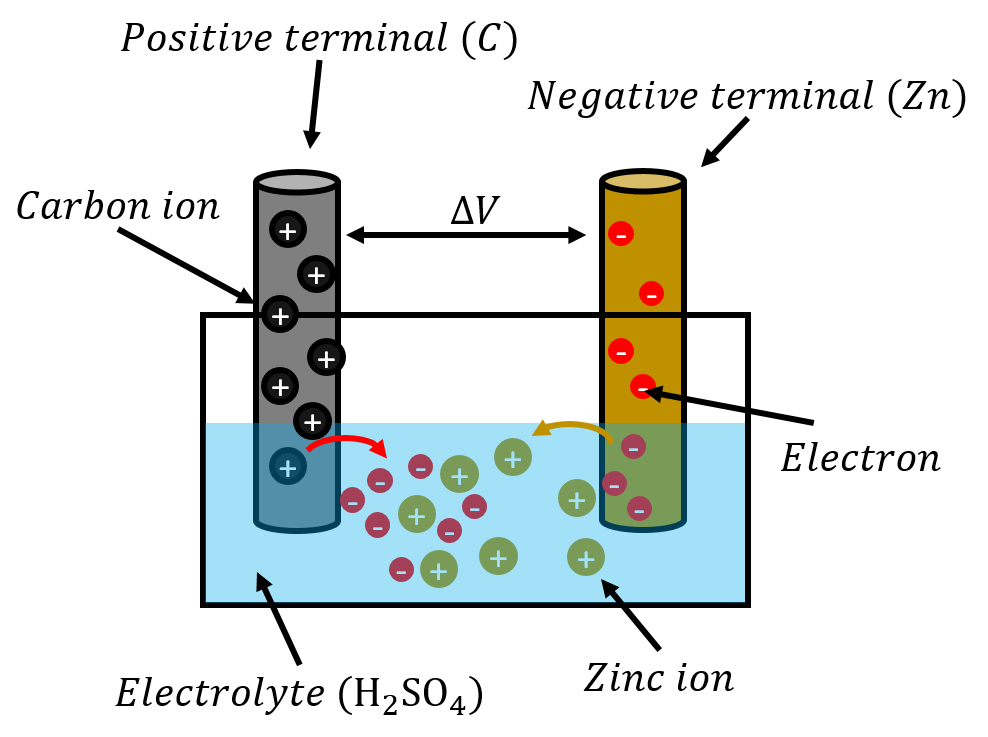
\includegraphics[width=0.7\linewidth]{files/electriccell-b624e62206c62803c9f633d00bae9bb0.png}
\caption[]{A simple electric cell, where zinc ions dissolve in sulfuric acid leaving electrons on the metal.}
\label{fig:circuits:electriccell}
\end{figure}

% TODO Is it incorrect to show the electrons entering the solution?

Once the zinc is immersed in the electrolyte, the zinc atoms tend to dissolve into the electrolyte in the form of zinc ions (doubly charged, Zn\textsuperscript{2+}). This leaves an excess of electrons on the zinc electrode, resulting in a net negative electric charge. Similarly, the positively charged zinc ions attract electrons from the carbon electrode into the solution, leaving the carbon electrode positively charged. Very quickly, an equilibrium is reached, since at some point, the negative charge of the zinc electrode will electrically attract positive zinc ions, preventing any more zinc ions from dissolving into the solution. Similarly, as the carbon electrode builds a positive charge, that charge will eventually prevent electrons from ``jumping'' into the solution. At this point, there will be a fixed electric potential difference between the two electrodes (terminals) of the battery.

If the two electrodes are connected together through a resistor, the electrons will leave the zinc electrode, cross the resistor, and end up on the positive carbon electrode. This will leave space for more electrons on the zinc electrode, so more zinc ions will dissolve into the solution. Thus, a circuit is formed, where electron travel up the zinc electrode, through the resistor and back down the carbon electrode. At the same time, more and more zinc ions dissolve into the electrolyte, until the zinc electrode is completely dissolved. In practice, the zinc ions travel through the solution and plate onto the carbon electrode (the electrons do not quite ``jump'' into the electrolyte, rather, it is the zinc ions that move in the electrolyte). Since the charge on the electrodes is continuously replenished, the potential difference between the electrodes remains constant even as current is flowing.

The electric cell will stop working once the zinc electrode has completely dissolved (this is what happens when your battery is dead). Note that there is also a maximum current that the cell can supply, which depends on the rate at which the zinc can dissolve into the electrolyte and plate onto the carbon electrode. If the electrodes of the cell are connected with a very low resistance resistor, the resulting current will be too large for the potential difference to be maintained. Most electric cells work in similar ways, although the chemical reactions can be much more complex. Sometimes, the chemical reaction is reversible; one could use a different battery to apply a negative voltage to the carbon electrode to reverse the reaction and plate the zinc back onto the zinc electrode, thus ``recharging the battery'' (and converting electric energy back into stored chemical potential energy).

\paragraph{The ideal battery in a circuit}

As we proceed, we will use the term ``battery'' loosely to refer to a device (such as an electric cell or collection of cells) that can provide a fixed potential difference between two terminals (or electrodes). Figure~\ref{fig:circuits:batterysymbol} shows the circuit diagram for a battery, consisting of two (or four) vertical bars, with the larger bar indicating the positive terminal of the battery.

\begin{figure}[!htbp]
\centering
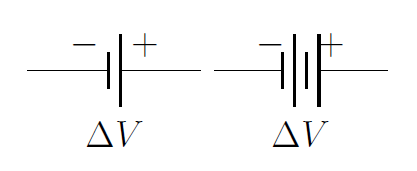
\includegraphics[width=0.6\linewidth]{files/batterysymbol-274afa3da108a9466ac4272b2cd962c5.png}
\caption[]{Circuit diagram symbols that can be used for a battery.}
\label{fig:circuits:batterysymbol}
\end{figure}

Figure~\ref{fig:circuits:resistorsymbol} shows the circuit diagram symbols that are used for a resistor (different symbols are used in North American and in Europe).

\begin{figure}[!htbp]
\centering
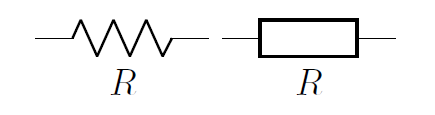
\includegraphics[width=0.6\linewidth]{files/resistorsymbol-cdfd7783ebc9bea4d3ca2eec6411d202.png}
\caption[]{Circuit diagram symbols for a resistor, using the North American convention (left), and the European convention (right).}
\label{fig:circuits:resistorsymbol}
\end{figure}

Figure~\ref{fig:circuits:batteryresistor} shows a circuit diagram for a very simple circuit consisting of a single $9 {\rm V}$ battery connected to a $2 {\rm \Omega}$ resistor. When drawing a circuit diagram (or making a real circuit), one connects the various components together (e.g. batteries and resistors) with \textbf{segments of wire that have zero resistance}, even if, in practice, wires always have some resistance. However, since the wires are connected in series with resistors (or other components that have a resistance), one can always include the resistance of the wires by adding it to the resistance of the other components. For example, in Figure~\ref{fig:circuits:batteryresistor}, if the wires have a total resistance of $1 {\rm \Omega}$, we could simply model the circuit as if the resistor had a resistance of $3 {\rm \Omega}$ instead of $2 {\rm \Omega}$. In practice, this is usually accounted for when a circuit diagram is made (i.e. any resistors include the resistance of the wires connected to it).

\begin{figure}[!htbp]
\centering
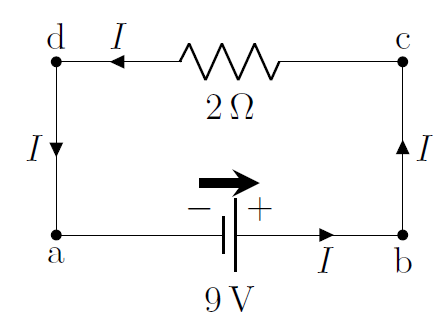
\includegraphics[width=0.35\linewidth]{files/batteryresistor-2b2416149cc3b585879ef82a83e4ac22.png}
\caption[]{A simple circuit, showing a $9 {\rm V}$ battery and a $2 {\rm \Omega}$ resistor. For ease in analyzing circuits, we suggest drawing a ``battery arrow" above batteries that goes from the negative to the positive terminal.}
\label{fig:circuits:batteryresistor}
\end{figure}

The circuit in Figure~\ref{fig:circuits:batteryresistor} is simple to analyze. In this case, whichever charges exit one terminal of the battery must pass through the resistor and then enter the other terminal of the battery. We \textbf{always use conventional current} to analyze a circuit. Thus, we model the circuit as if positive charges exit the positive terminal of the battery, go through the resistor, and then enter the negative terminal of the battery.

We recommend that you always draw a ``battery arrow'' for each battery in a circuit diagram to indicate the direction in which the electric potential increases and in which direction the conventional current would exit the battery if a simple resistor were connected across the battery. We also indicate the current that is flowing in any wire of the circuit by drawing an arrow in the direction of current on that wire (labelled $I$ in Figure~\ref{fig:circuits:batteryresistor}).

% In complex circuits, the current may not necessarily flow in the same direction as the battery arrow, and the battery arrow makes it easier to analyze those circuits.

It is helpful to think about the value of the electric potential along different parts of a circuit. Below (Figure~\ref{fig:circuits:batteryresistor_colour}), we have taken the circuit from Figure~\ref{fig:circuits:batteryresistor} and highlighted regions where the electric potential is constant.

\begin{figure}[!htbp]
\centering
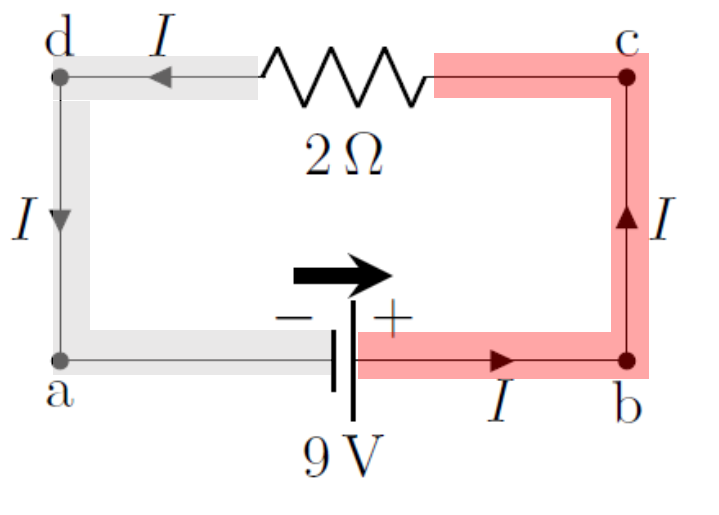
\includegraphics[width=0.4\linewidth]{files/batteryresistor_colo-947aa7e3376cf4c2c40889a8b3e04443.png}
\caption[]{The same circuit as in Figure~\ref{fig:circuits:batteryresistor} showing the two regions over which the electric potential is constant.}
\label{fig:circuits:batteryresistor_colour}
\end{figure}

Since the wires have no resistance, the electric potential is constant along a wire. In other words, because the wire has no resistance, the charges/current cannot dissipate any power in the wire ($P=I^2R$), and the charges do not ``lose'' any potential energy (and so the potential cannot change). The only place where the charges can dissipate energy is inside the resistor. Once the charges have crossed the resistor, the electric potential in the wire is again constant until they reach the other terminal of the battery. Thus, in this simple circuit, the electric potential difference across the resistor is the same as the potential difference across the terminals of the battery.  This is shown by the coloured areas in Figure~\ref{fig:circuits:batteryresistor_colour}. If we choose $0 {\rm V}$ to be defined at the negative terminal of the battery, then the potential is $9 {\rm V}$ everywhere in the red area (to the right of the resistor), and $0 {\rm V}$ everywhere in the grey area (to the left of the resistor).

We can apply Ohm's Law (the macroscopic version) to the resistor and determine the current in the circuit, since we know the potential difference across the resistor:
\begin{equation}
\Delta V&=RI\\
\therefore I&=\frac{\Delta V}{R}=\frac{(9 {\rm V})}{(2 {\rm \Omega})}=4.5 {\rm A}
\end{equation}

It is helpful to think of circuits in terms of energy. Charges move along the circuit and their potential energy changes as they go through components, while it remains constant as they move through a wire. If a positive charge enters the negative terminal of a battery and exits the positive terminal, its potential energy will have increased. If that charge then enters a resistor, its potential energy will decrease as it moves through the resistor, since the charge will ``use'' its potential energy to heat up the resistor. Batteries provide the energy to ``push'' the charges through the resistors in the circuit by converting chemical potential energy into the electrical potential energy of the charges.

It is also useful to make the analogy with fluid dynamics; one can think of the battery as a pump that is continuously pushing a viscous incompressible fluid through a pipe with a narrow section, as illustrated in Figure~\ref{fig:circuits:watercircuit}. The wide section of the pipe is akin to the wires with no resistance, and the narrow section is akin to the resistor. The pressure difference generated by the pump is analogous to the voltage produced by the battery, and the flow rate of the liquid is analogous to the electric current. The pressure in the pipe does not drop in the wide section, if there is no resistance. The entire pressure drop of the fluid is across the narrow section, just as the voltage only drops across the resistor.

\begin{figure}[!htbp]
\centering
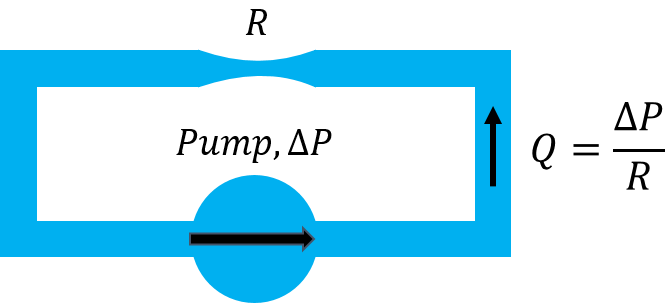
\includegraphics[width=0.5\linewidth]{files/watercircuit-c2d85239697efc723170b761c8b1073a.png}
\caption[]{A fluid dynamics analogue of the circuit in Figure~\ref{fig:circuits:batteryresistor}, where a pump plays the role of the battery, and a narrow pipe that of a resistor.}
\label{fig:circuits:watercircuit}
\end{figure}

\begin{framed}
\textbf{Example 19.1}\\
Two resistors, of $2 {\rm \Omega}$ and $4 {\rm \Omega}$, respectively, are connected in series to a $12 {\rm V}$ battery. What is the current through each of the resistors, and what is the voltage across each resistor?

\begin{framed}
\textbf{Solution}\\
We start by making a circuit diagram, as in Figure~\ref{fig:circuits:tworesistors}, showing the resistors, the current, $I$, the battery and the battery arrow. Note that since this is a closed circuit with only one path, the current through the battery, $I$, is the same as the current through the two resistors.

\begin{figure}[!htbp]
\centering
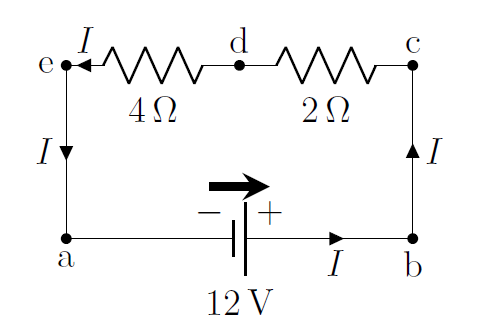
\includegraphics[width=0.42\linewidth]{files/tworesistors-e49d8c6bd8a4e07e755b86fd2da0ea23.png}
\caption[]{Two resistors connected in series with a battery.}
\label{fig:circuits:tworesistors}
\end{figure}

If we choose the potential on the negative side of the battery to be $0 {\rm V}$, then points ${\rm a}$ and ${\rm e}$ on the diagram are at a potential of $0 {\rm V}$, since potential cannot change in a wire with no resistance. Similarly, the points at ${\rm b}$ and ${\rm c}$ are at a potential of $12 {\rm V}$ (relative to points ${\rm a}$ and ${\rm e}$). At point ${\rm d}$, between the two resistors, the potential will be between $0 {\rm V}$ and $12 {\rm V}$, since the potential will ``drop'' as the current goes through the $2 {\rm \Omega}$ resistor.

The easiest way to determine the current through this simple circuit is to combine the two resistors into a single effective resistor with resistance:
\begin{equation}
R_{eff}=(2 {\rm \Omega})+(4 {\rm \Omega})=6 {\rm \Omega}
\end{equation}
so that the circuit can be simplified to that shown in Figure~\ref{fig:circuits:batteryresistor2}:

\begin{figure}[!htbp]
\centering
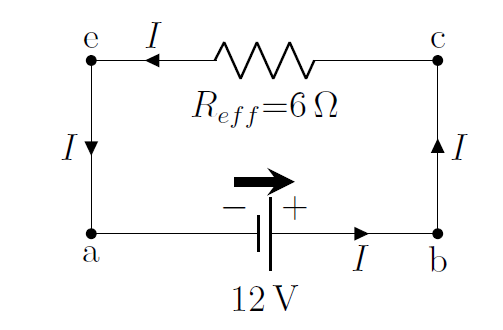
\includegraphics[width=0.42\linewidth]{files/batteryresistor2-ec040ff635391cdcdeeaef863ed15370.png}
\caption[]{The resistors from the circuit in Figure~\ref{fig:circuits:tworesistors} have been combined in series to simplify the circuit.}
\label{fig:circuits:batteryresistor2}
\end{figure}

The potential difference across the effective resistor is the same as that across the battery (between points ${\rm e}$ and ${\rm c}$), so that Ohm's Law can be applied to the effective resistor to determine the current that traverses it:
\begin{equation}
\Delta V &= R_{eff}I\\
\therefore I&=\frac{\Delta V}{R_{eff}}=\frac{(12 {\rm V})}{(6 {\rm \Omega})}=2 {\rm A}
\end{equation}
This current is the same that traverses each individual resistor, since it is the same as the current that goes through the battery. Referring back to the full circuit (Figure~\ref{fig:circuits:tworesistors}), we can now use Ohm's Law to calculate the voltage drop across each resistor, since we know the current through each resistor. The voltage across the $2 {\rm \Omega}$ resistor is given by:
\begin{equation}
\Delta V_{2\Omega}=RI=(2 {\rm \Omega})(2 {\rm A})=4 {\rm V}
\end{equation}
and the voltage across the $4 {\rm \Omega}$ resistor is given by:
\begin{equation}
\Delta V_{4\Omega}=RI=(4 {\rm \Omega})(2 {\rm A})=8 {\rm V}
\end{equation}
Note that the sum of these two voltages is equal to the voltage increase across the battery, by conservation of energy. Consider the electric potential at different points in Figure~\ref{fig:circuits:tworesistors} as you move clockwise around the loop starting at point ${\rm a}$. If the electric potential is defined to be $0 {\rm V}$ at the negative end of the battery (points ${\rm a}$ and ${\rm e}$), the potential at point ${\rm d}$ (between the resistors) is the potential at point ${\rm e}$ plus the potential difference across the $4 {\rm \Omega}$ resistor:
\begin{equation}
V_d = V_e+\Delta V_{4\Omega}=(0 {\rm V})+(\Delta V_{4\Omega})=8 {\rm V}
\end{equation}
If we then add the potential difference across the $2 {\rm \Omega}$ resistor to the potential at point ${\rm d}$, we find  that the potential at point ${\rm c}$ is $V_c=V_d+\Delta V_{2\Omega}=12 {\rm V}$, as expected, since this corresponds to the potential at the positive terminal of the battery.

\textbf{Discussion:} In this example, we showed how one can model a circuit by combining resistors together into effective resistors to simplify the circuit. We also showed how the potential differences across different components in a circuit must add up to zero (the voltage drops across the resistors must sum to the voltage increase across the battery).
\end{framed}
\end{framed}

\begin{framed}
\textbf{Checkpoint}\\
What is the voltage across the combination of a $3 {\rm V}$ battery connected in series with a $6 {\rm V}$ battery, where the negative terminal of the $6 {\rm V}$ battery faces the positive terminal of the $3 {\rm V}$ battery?

\begin{enumerate}
\item $9 {\rm V}$.
\item $6 {\rm V}$.
\item $3 {\rm V}$.
\item $0 {\rm V}$.
\end{enumerate}

\begin{framed}
\textbf{Answer}\\
\begin{enumerate}
\item
\end{enumerate}
\end{framed}
\end{framed}

\paragraph{The real battery in a circuit}

So far, we have modelled batteries as ``ideal'' devices that provide a fixed potential difference. In reality, this neglects the fact that the materials that make the battery will themselves have a resistance. For example, if electrons want to leave the zinc rod in the electric cell illustrated in Figure~\ref{fig:circuits:electriccell}, they will lose some energy as they pass through the zinc. Thus, when modelling a real battery in a circuit, it is important to include its ``internal resistance'', as a resistor in series with the potential difference. This is illustrated in Figure~\ref{fig:circuits:realbattery}, which shows the two terminals of a real battery, an ideal battery (with a fixed potential difference, $\Delta V_{ideal}$), and its internal resistance, $r$ (which can be drawn on either side of the battery).

\begin{figure}[!htbp]
\centering
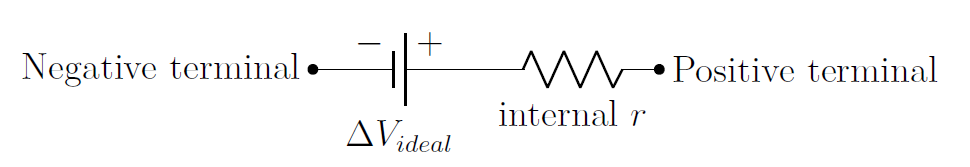
\includegraphics[width=0.8\linewidth]{files/realbattery-25df902f5102763e8da286f2d44bddb1.png}
\caption[]{Model of a real battery, showing an ideal battery in series with a resistor to model the internal resistance of the battery.}
\label{fig:circuits:realbattery}
\end{figure}

It is important to note that the potential difference across the terminals of the real battery is only equal to the potential difference across the ideal battery \textbf{if there is no current flowing through the battery}. If there is a current, $I$, flowing through the internal resistance, the electric potential will decrease by an amount $Ir$ across the internal resistance, and the voltage across the real terminals will be $\Delta V_{ideal} -Ir$.

\begin{framed}
\textbf{Example 19.2}\\
When no resistance is connected across a real battery, the potential difference across its terminals is measured to be $6 {\rm V}$. When an $R=2 {\rm \Omega}$ resistor is connected across the battery, a current of $2 {\rm A}$ is measured through the resistor. What is the internal resistance, $r$, of the battery, and what is the voltage across its terminals when the $R=2 {\rm \Omega}$ resistor is connected?

\begin{framed}
\textbf{Solution}\\
The real battery can be modelled as an ideal battery with potential difference, $\Delta V_{ideal}$, in series with an internal resistance, $r$. While we do not know the value of the internal resistance, we are told that the potential difference across the terminals of the real battery is $6 {\rm V}$ \textbf{when no current flows through it}. Since no current flows through the internal resistance, the voltage does not drop across the internal resistance, and the voltage across the terminals of the real battery (e.g. Figure~\ref{fig:circuits:realbattery}) must thus be equal to the voltage across the terminals of the ideal battery, so that $\Delta V_{ideal}=6 {\rm V}$.

With this information, we can make a circuit diagram for the case when the $2 {\rm \Omega}$ resistor is connected across the terminals of the real battery, as in Figure~\ref{fig:circuits:realbatterycircuit}.

\begin{figure}[!htbp]
\centering
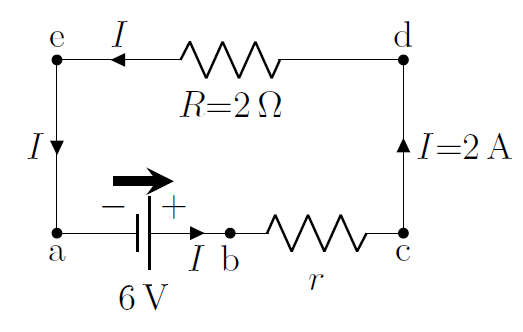
\includegraphics[width=0.42\linewidth]{files/realbatterycircuit-c0da95c1617d5d17aee894d81382d86a.png}
\caption[]{A circuit showing a real battery (with internal resistance $r$) in series with a resistor.}
\label{fig:circuits:realbatterycircuit}
\end{figure}

The terminals of the real battery are located at points ${\rm a}$ and ${\rm c}$ of the diagram, whereas the terminals of the ideal battery correspond to points ${\rm a}$ and ${\rm b}$. When no current flows through the internal resistor, $r$, there is no voltage drop across that resistor and the potential at ${\rm b}$ will be equal to the potential at ${\rm c}$, as we argued above.

The circuit in Figure~\ref{fig:circuits:realbatterycircuit} is now identical to that analyzed in Example~19.1, and can be treated the same way. We can combine the $2 {\rm \Omega}$ resistor with the internal resistance, $r$, in series to obtain an effective resistor, $R_{eff}=r+R$. The voltage drop across the effective resistor will be the same as the potential difference across the ideal battery, and we can make use of Ohm's Law to find the internal resistance, $r$:
\begin{equation}
\Delta V_{ideal}&= R_{eff}I=(r+R)I\\
\therefore r &= \frac{\Delta V_{ideal}}{I}-R=\frac{(6 {\rm V})}{(2 {\rm A})}-(2 {\rm \Omega})=1 {\rm \Omega}
\end{equation}
Now that we know the internal resistance, we can determine the voltage drop across the internal resistor, using Ohm's Law:
\begin{equation}
\Delta V_r = rI=(1 {\rm \Omega})(2 {\rm A})=2 {\rm V}
\end{equation}
The voltage drop across the real terminals of the battery (between points ${\rm a}$ and ${\rm c}$), is thus given by:
\begin{equation}
\Delta V_{real}=\Delta V_{ideal}-\Delta V_r=(6 {\rm V})-(2 {\rm V})=4 {\rm V}
\end{equation}
Again, you can verify that the voltage drops across the two resistors will sum to the total voltage drop across the terminals of the ideal battery.

\textbf{Discussion:} Modelling real batteries is not so different from modelling ideal batteries, since one only needs to include an internal resistance into the circuit. The key difference with a real battery is that the voltage across its real terminals depends on what is connected to the battery. In the example above, the battery has a voltage of $6 {\rm V}$ across its (real) terminals when nothing is connected, but the voltage drops to $4 {\rm V}$ when a $2 {\rm \Omega}$ resistor is connected.
\end{framed}
\end{framed}

\begin{framed}
\textbf{Checkpoint}\\
Suppose that you would like to measure the ideal voltage of a real battery by connecting a measurement device (a voltmeter) across its terminals. In order to get the most accurate reading, should you choose a voltmeter with a high resistance, or a voltmeter with a low resistance?

\begin{enumerate}
\item High resistance.
\item Low resistance.
\item It doesn't matter if the voltmeter has a high or low resistance.
\end{enumerate}

\begin{framed}
\textbf{Answer}\\
\begin{enumerate}
\item
\end{enumerate}
\end{framed}
\end{framed}

\subsubsection{Kirchhoff's rules}

Kirchhoff's rules correspond to concepts that we have already covered, but allow us to easily model more complex circuits, for instance, those where there is more than one path for the current to take. Kirchhoff's rules refer to ``junctions'' and ``loops''. Junctions and loops depend only on the shape of the circuit, and not on the components in the circuit. Figure~\ref{fig:circuits:3loopempty} shows a circuit with no components in order to illustrate what is meant by a junction and a loop.

\begin{figure}[!htbp]
\centering
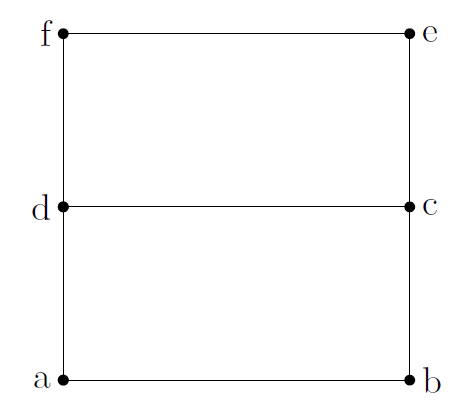
\includegraphics[width=0.4\linewidth]{files/3loopempty-0e9cf961ed755afb96b62a98e97680bd.png}
\caption[]{A circuit that has 3 loops and 2 junctions.}
\label{fig:circuits:3loopempty}
\end{figure}

The locations at points ${\rm d}$ and ${\rm c}$ are considered ``junctions'', because there are more than 2 segments of wire connected to that point. The points at locations ${\rm a}$, ${\rm b}$, ${\rm e}$ and ${\rm f}$ only have two segments of wire connected to them. The circuit in Figure~\ref{fig:circuits:3loopempty} thus has 2 junctions.

A loop is a closed path that one can trace around the circuit without passing over the same segment of wire twice. The circuit in Figure~\ref{fig:circuits:3loopempty} has 3 such loops, which we can identify using the letters at the various nodes of the circuit:

\begin{enumerate}
\item ${\rm abcda}$
\item ${\rm abcefda}$
\item ${\rm dcefd}$
\end{enumerate}

Note that it does not matter where one starts on the loop, only that one can identify how many different loops are present in the circuit.

% %%The loops are shown more explicitly in [](#fig:circuits:looplabel).%%%
% %%```{figure} figures/Circuits/circuitspng/looplabel.png
% %%:label: fig:circuits:looplabel
% %%:width: 40%
% %%:align: center
% %%:alt: The three loops in the circuit.
% %%The three loops in the circuit.
% %%```

\begin{framed}
\textbf{Checkpoint}\\
\begin{figure}[!htbp]
\centering
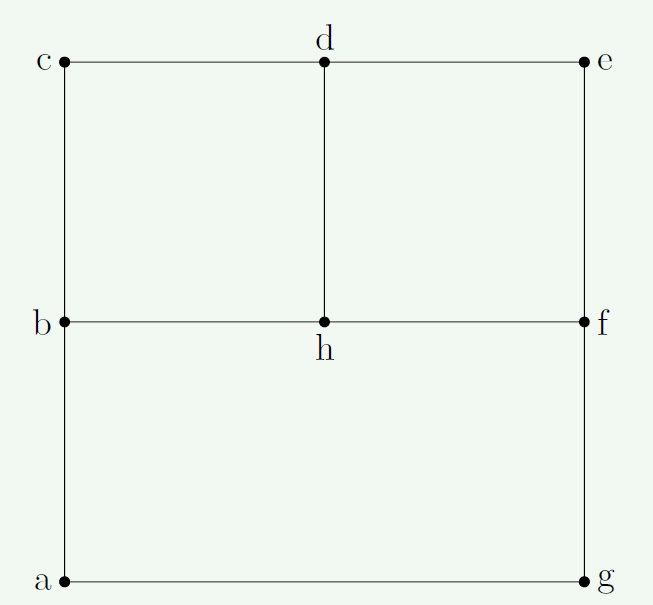
\includegraphics[width=0.5\linewidth]{files/7loop-7d21110540d72f12bf874c92522b5941.png}
\caption[]{Circuit layout}
\label{fig:circuits:7loop}
\end{figure}

How many loops and junctions does the circuit in Figure~\ref{fig:circuits:7loop} have?

\begin{enumerate}
\item The circuit has five loops and four junctions
\item The circuit has three loops and eight junctions
\item The circuit has seven loops and four junctions.
\item The circuit has four loops and four junctions.
\end{enumerate}

\begin{framed}
\textbf{Answer}\\
\begin{enumerate}[resume]
\item
\end{enumerate}
\end{framed}
\end{framed}

\paragraph{Junction rule}

The junction rule states that: \textbf{The current entering a junction must be equal to the current exiting a junction.}

This is in fact a simple statement about conservation of charge. If charges are flowing into a junction (from one or more segments of wire in that junction), then the same amount of charges must flow back out of the junction (through one or more different segments of wire).

Consider the junction illustrated in Figure~\ref{fig:circuits:junction}, comprised of 5 segments of wire, each carrying a different current. As shown, currents $I_1$, $I_3$, and $I_4$ flow into the junction, whereas currents $I_2$ and $I_5$ flow out of the junction.

\begin{figure}[!htbp]
\centering
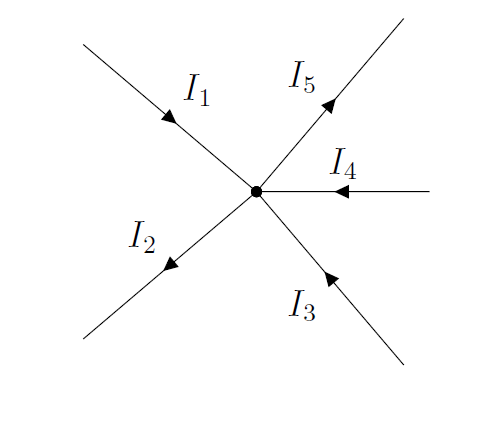
\includegraphics[width=0.4\linewidth]{files/junction-4828061de9aa07ebe924a9a7d3495dbf.png}
\caption[]{A junction with 5 segments and 5 currents.}
\label{fig:circuits:junction}
\end{figure}

The junction rule states that the current entering the junction must equal the current coming out of the junction. This allows us to relate the currents to each other in an equation:
\begin{equation}
\text{incoming currents}&=\text{outgoing currents}\\
I_1+I_3+I_4 &=I_2+I_5
\end{equation}

\paragraph{Loop rule}

The loop rule states that: \textbf{The net voltage drop across a loop must be zero.}

This is a statement about conservation of energy, that we already noted in Example~19.1. Once you have identified a specific loop, if you trace a closed path around the loop, the electric potential must be the same at the end of the path as at the beginning of the path (since it is literally the same point in space). This means that if there is a voltage drop along the path (e.g. due to one or more resistors), then there must be equivalent voltage increases somewhere else on the path (e.g. due to one or more batteries). If this were not the case, it would be possible to have a path where charges could gain a net amount of energy by going around that path, which they could keep doing indefinitely and create an infinite amount of energy; instead, if charges gain potential energy in a battery, they must then lose exactly the same amount of energy inside one or more resistors along the path.

Figure~\ref{fig:circuits:loop} shows a loop (which could be part of a larger circuit) to which we can apply the loop rule. The loop contains two batteries, facing in opposite directions (which would not normally be a good use of batteries), as illustrated by the battery arrows.

\begin{figure}[!htbp]
\centering
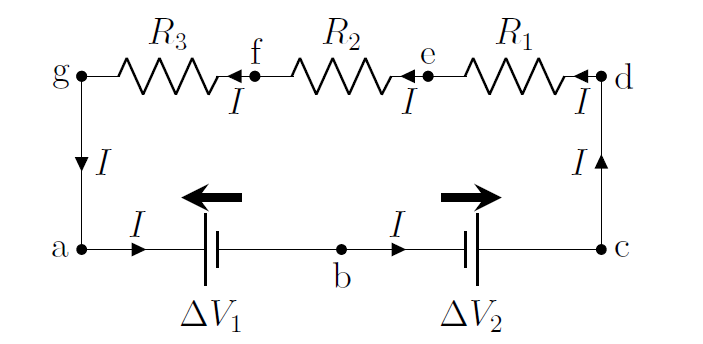
\includegraphics[width=0.55\linewidth]{files/loop-ad77847ada097ce589459094edc79d1b.png}
\caption[]{A loop with 2 batteries and 3 resistors.}
\label{fig:circuits:loop}
\end{figure}

The procedure for applying the loop rule is as follows:

\begin{enumerate}
\item Identify the loop, including starting position and direction.
\item Start at the beginning of the loop, and trace around the loop.
\item Each time a battery is encountered, \textbf{add the battery voltage if you are tracing the loop in the same direction as the corresponding battery arrow}, subtract the voltage otherwise.
\item Each time a resistor is encountered, \textbf{subtract the voltage across that resistor ($RI$, from Ohm's Law) if tracing the loop in the same direction as the current}, add the the voltage otherwise.
\item Once you have traced back to the starting point, the resulting sum must be zero.
\end{enumerate}

To illustrate the procedure, we trace out the loop ${\rm abcedfga}$ in Figure~\ref{fig:circuits:loop}. We thus start at point ${\rm a}$ and trace the loop in the counter-clockwise direction.

\begin{itemize}
\item Between points ${\rm a}$ and ${\rm b}$ we encounter a battery, and we are tracing in the \textbf{opposite direction of that battery's arrow}, so we subtract the voltage from that battery: $-\Delta V_1$.
\item Between points ${\rm b}$ and ${\rm c}$, we encounter a battery, and we are tracing in the \textbf{same direction as that battery's arrow}, so we add the voltage from that battery: $+\Delta V_2$.
\item Nothing happens to the potential along the wire from ${\rm c}$ to ${\rm d}$.
\item Between points ${\rm d}$ and ${\rm e}$, we encounter a resistor, and we are tracing in the \textbf{same direction as the current through that resistor}, so subtract the voltage across that resistor: $-R_1I$).
\item Similarly, we subtract the voltages across resistors $R_2$ and $R_3$, as we are tracing in the \textbf{same direction as the current through those resistors}: $-IR_2 -IR_3$.
\item We are back at the beginning of the loop, so the terms must sum to zero.
\end{itemize}

We can now use the loop rule, which states that the sum of the above voltages must be zero:
\begin{equation}
-\Delta V_1 + \Delta V_2 - R_1I - R_2I - R_3I = 0\quad \text{(loop abcdefga)}
\end{equation}
This equation then gives us a relation between the various quantities (current, resistors, battery voltages) in the circuit which can be used to model the circuit.

\begin{framed}
\textbf{Checkpoint}\\
Suppose that the equation describing loop ${\rm abcdefga}$ (Figure~\ref{fig:circuits:loop}) was obtained from a different starting position and the loop was traced in the opposite direction. Would this produce a different equation?

\begin{enumerate}
\item Yes, the equation would be incorrect if the loop is traced in the direction opposite to the flow of current.
\item Yes, the equation must start from the point ${\rm a}$ because the creator of the circuit assumes the person calculating current and voltage will begin at point ${\rm a}$.
\item Yes, there is no incorrect starting point, but choosing to trace the circuit in the direction opposite to the flow of current would produce an incorrect equation.
\item No, there is no incorrect direction or starting point.
\end{enumerate}

\begin{framed}
\textbf{Answer}\\
\begin{enumerate}[resume]
\item
\end{enumerate}
\end{framed}
\end{framed}

\begin{framed}
\textbf{Olivia's Thoughts}\\
One way to conceptualize Kirchhoff's loop rule is to draw an analogy to gravity. Imagine that the circuit in Figure~\ref{fig:circuits:loop} operates like a roller coaster, as shown in Figure~\ref{fig:circuits:rollercoaster}. Each battery is like the mechanical lift that brings the cart to the top of the hill. The battery arrow points in the uphill direction.

\begin{figure}[!htbp]
\centering
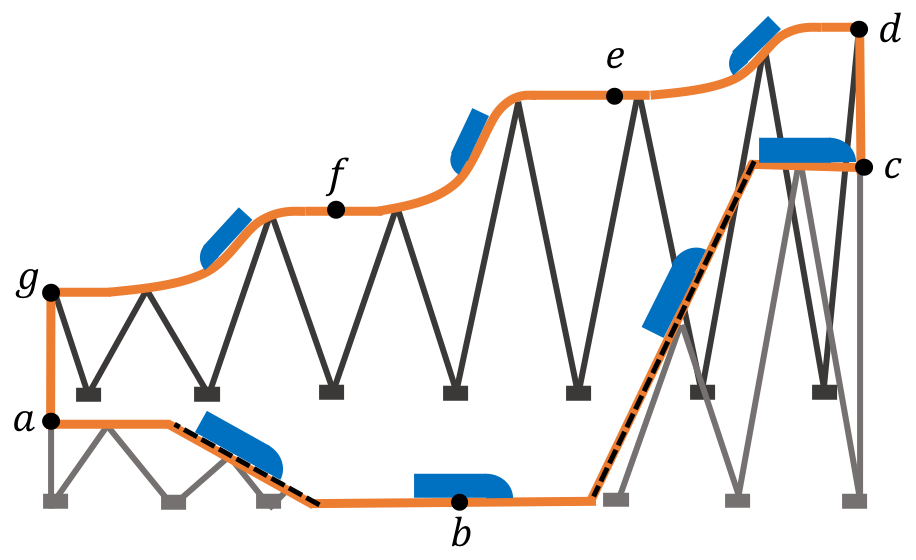
\includegraphics[width=0.5\linewidth]{files/rollercoaster-30ac3b258fc22d96ce9b0086f3ceaa74.png}
\caption[]{The circuit from Figure~\ref{fig:circuits:loop} using the roller coaster analogy.}
\label{fig:circuits:rollercoaster}
\end{figure}

This time, we'll start at point ${\rm b}$ and go counter clockwise. In this analogy, Kirchhoff's loop rule says that when the roller coaster cart comes back around to ${\rm b}$, it needs to have the same gravitational potential it started with (since it will be at the same elevation). Let's follow its journey around the loop. It starts at ${\rm b}$, then goes through a battery and gets lifted uphill. The cart moves along the track (in the direction of the current) and loses potential energy whenever it goes down a hill (meaning through a resistor). When the cart comes around the left side of the circuit, it encounters another battery. This time, the cart is moving \textit{opposite} to the battery arrow, so the cart goes downhill instead of getting lifted uphill. When it gets back to ${\rm b}$, it has the same potential it started with. Note that, if we are moving in the direction opposite to the current, this is like going backwards through the roller coaster. Instead of going downhill through each resistor, you would have to go uphill, and thus gain potential energy.
\end{framed}

\subsubsection{Applying Kirchhoff's rules to model circuits}

In this section, we show how to model a circuit using Kirchhoff's rules. In general, one can consider a circuit to be fully modelled if one can determine the current in each segment of the circuit. We will show how one can apply the same procedure to model any circuit that contains batteries and resistors. The procedure is as follows:

\begin{enumerate}
\item Make a good diagram of the circuit.
\item Simplify any resistors that can easily be combined into effective resistors (in series or in parallel).
\item Make a new diagram with the effective resistors, showing battery arrows, and labelling all of the nodes so that loops can easily be described.
\item Make a \textbf{guess} for the directions of the current in each segment.
\item Write the junction rule equations.
\item Write the loop equations.
\item This will lead to $N$ independent equations that one can solve for the $N$ different currents in the circuit.
\item Once you have determined all of the currents, if some of them are negative numbers, switch the direction of those currents in the diagram (they will be negative if you guessed the direction incorrectly).
\end{enumerate}

We will illustrate the procedure on the circuit shown in Figure~\ref{fig:circuits:bigcircuit}, for which we would like to know the current through each resistor and each battery. The circuit contains 5 resistors ($R_1$-$R_5$), 2 real batteries (with ideal voltages $\Delta V_1$ and $\Delta V_2$), and 2 additional resistors to model the internal resistances of the real batteries ($r_1$, $r_2$)

\begin{figure}[!htbp]
\centering
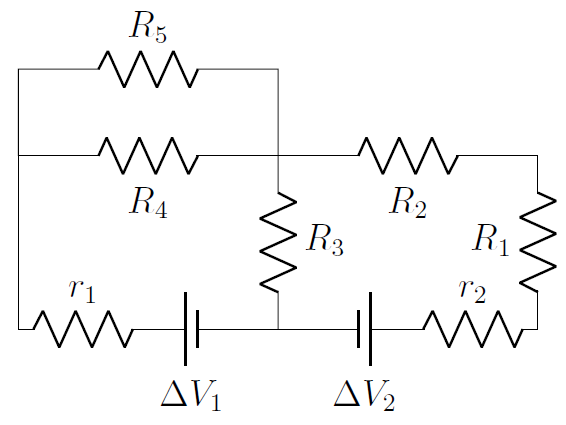
\includegraphics[width=0.42\linewidth]{files/bigcircuit-d85731ab6ffaa6e5a59fc67d56856ba0.png}
\caption[]{A circuit that can be simplified and then solved with Kirchhoff's rules.}
\label{fig:circuits:bigcircuit}
\end{figure}

\begin{framed}
\textbf{Checkpoint}\\
How many different currents are in the circuit shown in Figure~\ref{fig:circuits:bigcircuit}?

\begin{enumerate}
\item 3
\item 4
\item 5
\item 6
\end{enumerate}

\begin{framed}
\textbf{Answer}\\
\begin{enumerate}[resume]
\item
\end{enumerate}
\end{framed}
\end{framed}

\textbf{Simplifying the resistors (step 2):} In this circuit, resistors $r_2$, $R_1$ and $R_2$ are in series, so that they can be combined into an effective resistor, $R_6$:
\begin{equation}
R_6=r_2+R_1+R_2
\end{equation}
With this simplification, we obtain the circuit illustrated in Figure~\ref{fig:circuits:bigcircuit_simp1}

\begin{figure}[!htbp]
\centering
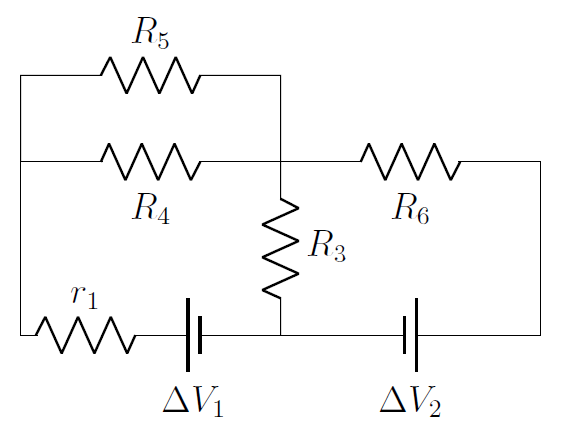
\includegraphics[width=0.42\linewidth]{files/bigcircuit_simp1-c3aa371fb88c44134be8c89020416c77.png}
\caption[]{The resistors $r_2$, $R_1$ and $R_2$ in series from the circuit in Figure~\ref{fig:circuits:bigcircuit} have been combined into the effective resistor, $R_6$, to simplify the circuit.}
\label{fig:circuits:bigcircuit_simp1}
\end{figure}

Next, we note that resistors $R_4$ and $R_5$ are in parallel and can be easily combined into a resistor, $R_7$:
\begin{equation}
R_7=\frac{R_4R_5}{R_4+R_5}
\end{equation}
which leads to the circuit illustrated in Figure~\ref{fig:circuits:bigcircuit_simp2}.

\begin{figure}[!htbp]
\centering
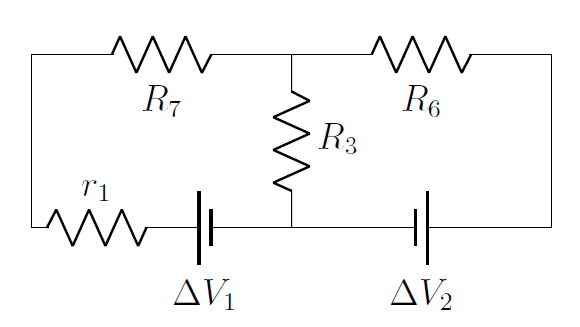
\includegraphics[width=0.42\linewidth]{files/bigcircuit_simp2-99756f76f2fb3356a4713b80fb3fb893.png}
\caption[]{The resistors $R_4$ and $R_5$ in parallel from the circuit in Figure~\ref{fig:circuits:bigcircuit_simp1} have been combined into the effective resistor, $R_7$, to simplify the circuit.}
\label{fig:circuits:bigcircuit_simp2}
\end{figure}

Finally, we note that $r_1$ and $R_7$ are in series and can be combined into an effective resistor, $R_8$:
\begin{equation}
R_8=r_1+R_7=r_1+\frac{R_4R_5}{R_4+R_5}
\end{equation}
leading to the simplified circuit illustrated in Figure~\ref{fig:circuits:bigcircuit_simp3}, which we have labelled with nodes and battery labels.

\begin{figure}[!htbp]
\centering
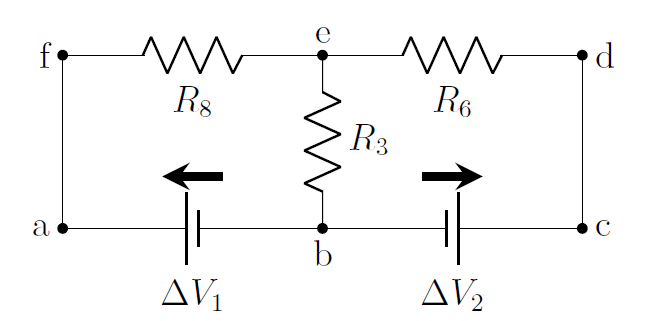
\includegraphics[width=0.45\linewidth]{files/bigcircuit_simp3-52981a5029c13508d012c4743b946805.png}
\caption[]{The resistors $r_1$ and $R_7$ from the circuit in Figure~\ref{fig:circuits:bigcircuit_simp2} have been combined into an effective resistor, $R_8$, to simplify the circuit.}
\label{fig:circuits:bigcircuit_simp3}
\end{figure}

\textbf{Guessing the directions of the currents (step 4):} Before we can write the equations from Kirchhoff's rules, we need to label the currents in the circuit diagram. In general, it is not always obvious in which way the currents will go, so we make a guess that we can fix later if we guessed wrong.

In order to guess the current directions, choose one point on the circuit and move along a segment. Label the current in that segment and continue moving through the circuit, splitting up the current when a junction is encountered. Make sure to only have one current per segment. We guess the currents as follows, referring to Figure~\ref{fig:circuits:bigcircuit_simp}:

\begin{itemize}
\item We start at point ${\rm a}$ and move upwards to point ${\rm f}$. We will call the current in that segment, $I_1$.
\item Since there is no junction, the current $I_1$ continues through the resistor $R_8$ to point ${\rm e}$.
\item There is a junction at point ${\rm e}$, so we split the current $I_1$ into currents $I_2$ (towards point ${\rm d}$), and $I_3$ (downwards to point ${\rm b}$).
\item We follow current $I_2$ first; $I_2$ flows from ${\rm e}$ to ${\rm d}$, then down to ${\rm c}$, through the battery $\Delta V_2$, and to point ${\rm b}$, where there is again junction.
\item We follow current $I_3$, which just flows down to the junction at point ${\rm b}$, where it ``meets up'' with current $I_2$.
\item Currents $I_2$ and $I_3$ both flow into the junction at point ${\rm b}$, and the current flowing out of the junction, through the battery $\Delta V_1$, and towards point ${\rm a}$ is, again, $I_1$, since this current then flows up to point ${\rm f}$.
\item All segments of wire have a labelled current, so we are done guessing currents.
\end{itemize}

You can proceed in an analogous way for any circuit. The final circuit, with currents labelled, is shown in Figure~\ref{fig:circuits:bigcircuit_simp}:

\begin{figure}[!htbp]
\centering
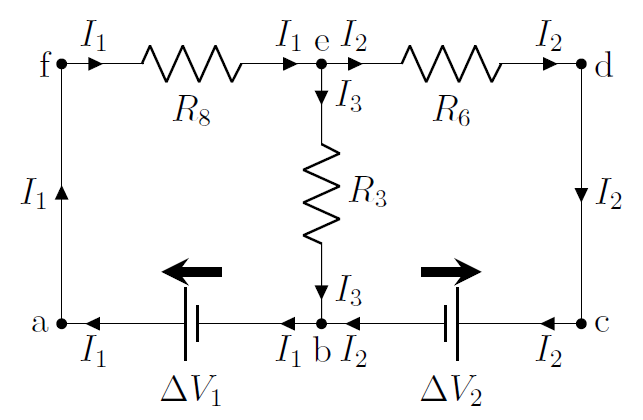
\includegraphics[width=0.45\linewidth]{files/bigcircuit_simp-74458b91bfc85d701204ec05fac2eb8a.png}
\caption[]{Final and labelled circuit diagram that is simplified from the one in Figure~\ref{fig:circuits:bigcircuit}.}
\label{fig:circuits:bigcircuit_simp}
\end{figure}

We can now proceed using Kirchhoff's rules to solve for the values of the currents in the circuit. It is useful to note that there are 3 unknown currents in this circuit; we thus hope that Kirchhoff's rules will give us 3 independent equations.

\textbf{Applying the junction rule (step 5):} In the circuit from Figure~\ref{fig:circuits:bigcircuit_simp}, there are two junctions (at points ${\rm b}$ and ${\rm e}$), so we will get two equations from the junction rule. To apply the junction rule, the sum of the currents coming into the junction must be equal to the currents going out of the junction:
\begin{equation}
\text{incoming currents}&=\text{outgoing currents}&\\
I_2+I_3 &= I_1 \quad &\text{(junction b)}\\
I_1 &= I_2+I_3 \quad &\text{(junction e)}\\
\end{equation}
Note that the two equations are not independent (in fact, they are the same). It is generally the case that if there $N$ junctions, one will obtain less than $N$ independent equations (usually, $N -1$ equations will be independent). In this case, the two junctions only gave us one equation.

\textbf{Applying the loop rule (step 6):} This circuit contains 3 different loops: ${\rm abcdefa}$, ${\rm abefa}$, and ${\rm bcdeb}$, which will lead to 3 equations from the loop rule. We expect that these equations will not be independent, since this would lead to 4 equations and 3 unknowns when combined with the junction rule equation. Let us start with the loop ${\rm abcdefa}$:

\begin{itemize}
\item From ${\rm a}$ to ${\rm b}$, we trace through the battery in the \textbf{opposite direction from the battery arrow}: $-\Delta V_1$.
\item From ${\rm b}$ to ${\rm c}$, we trace through the battery in the \textbf{same direction as the battery arrow}: $+\Delta V_2$.
\item From ${\rm c}$ through ${\rm d}$ and through to ${\rm e}$ we go through the resistor $R_6$ in the \textbf{opposite direction from the current}, $I_2$, in that resistor: $+I_2R_6$.
\item From ${\rm e}$ to ${\rm f}$, we go through the go through the resistor $R_8$ in the \textbf{opposite direction from the current}, $I_1$, in that resistor: $+I_1R_8$.
\item And we are back at the starting point, so the sum of the above terms is equal to zero.
\end{itemize}

which gives the equation:
\begin{equation}
-\Delta V_1+\Delta V_2+I_2R_6+I_1R_8=0\quad\text{(loop abcdefa)}
\end{equation}
Similarly, for the loop ${\rm abefa}$, we obtain:
\begin{equation}
-\Delta V_1+I_3R_3+I_1R_8=0\quad\text{(loop abefa)}
\end{equation}
and for loop ${\rm bcdeb}$:
\begin{equation}
\Delta V_2+I_2R_6-I_3R_3=0\quad\text{(loop bcdeb)}
\end{equation}
Although it appears that we have obtained 3 additional equations, only two of these are independent. For example, if you sum the second and third equations (loops ${\rm abefa}$, and ${\rm bcdeb}$), you simply obtain the first equation (loop ${\rm abcdefa}$). In general, if there are $N$ different loops, one will obtain less than $N$ independent equations (usually $N -1$ independent equations, as we did here).

At this point, after choosing one of the junction equations, and two of the loop equations, we have 3 independent equations that we can solve for the 3 unknown currents{\textbackslash}footnote\{The 3 unknowns do not necessarily have to be the currents, and could be any combination of the currents, battery voltage and resistors. As long as there at most 3 unknown quantities, this circuit can be solved.\}:
\begin{equation}
I_1 &= I_2+I_3 \quad &\text{(junction e)}\\
-\Delta V_1+\Delta V_2+I_2R_6+I_1R_8&=0\quad&\text{(loop abcdefa)}\\
-\Delta V_1+I_3R_3+I_1R_8&=0\quad&\text{(loop abefa)}
\end{equation}
It is only a matter of some simple math to solve for the 3 unknowns from these 3 equations (which we carry out in the example below).

\begin{framed}
\textbf{Example 19.3}\\
Referring to the circuit in Figure~\ref{fig:circuits:bigcircuit_vals}, what is the voltage across the real terminal of the battery with ideal voltage $\Delta V_1$ (the voltage between points ${\rm a}$ and ${\rm b}$)? What is the current through resistor $R_5$?

\begin{framed}
\textbf{Solution}\\
\begin{figure}[!htbp]
\centering
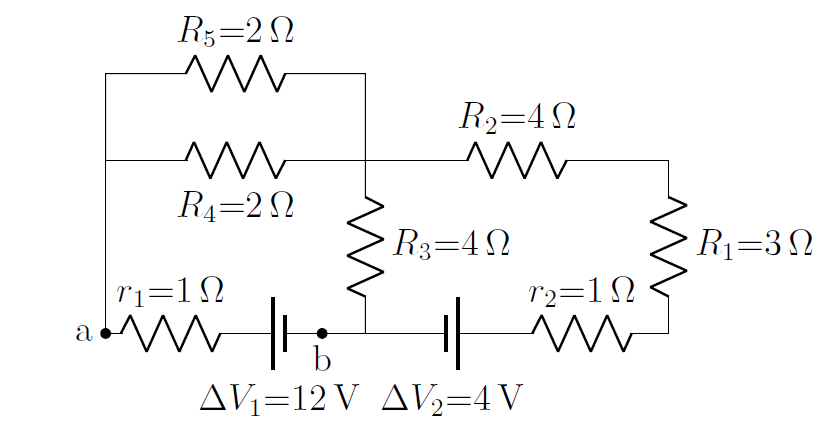
\includegraphics[width=0.6\linewidth]{files/bigcircuit_vals-5027390ef3ef30e202afcf35ff92a3fc.png}
\caption[]{The same circuit as in Figure~\ref{fig:circuits:bigcircuit}, with values filled in.}
\label{fig:circuits:bigcircuit_vals}
\end{figure}

Since this circuit is the same that we just analyzed, we know that it can be simplified into the circuit shown in Figure~\ref{fig:circuits:bigcircuit_vals_simp}, with resistors:
\begin{equation}
R_6&=r_2+R_1+R_2=(1 {\rm \Omega})+(3 {\rm \Omega})+(4 {\rm \Omega})=8 {\rm \Omega}\\
R_8&=r_1+\frac{R_4R_5}{R_4+R_5}=(1 {\rm \Omega})+\frac{(2 {\rm \Omega})(2 {\rm \Omega})}{(2 {\rm \Omega})+(2 {\rm \Omega})}=2 {\rm \Omega}
\end{equation}

\begin{figure}[!htbp]
\centering
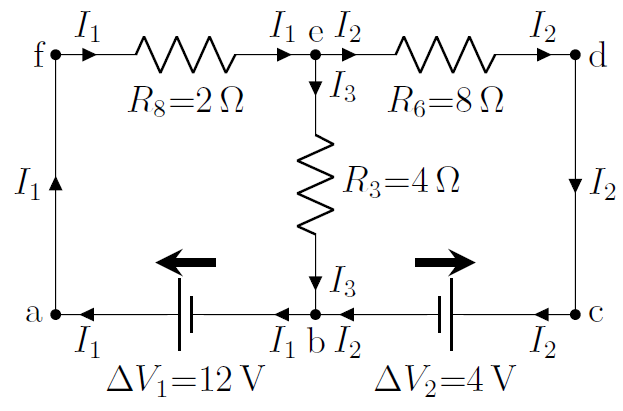
\includegraphics[width=0.45\linewidth]{files/bigcircuit_vals_simp-425edb9cdde8849007b8f6c25e9b96b5.png}
\caption[]{Simplified version of the circuit in Figure~\ref{fig:circuits:bigcircuit_vals}.}
\label{fig:circuits:bigcircuit_vals_simp}
\end{figure}

From above, we know that this leads to the following three equations:
\begin{equation}
I_1 &= I_2+I_3 \quad &\text{(junction e)}\\
-\Delta V_1+\Delta V_2+I_2R_6+I_1R_8&=0\quad&\text{(loop abcdefa)}\\
-\Delta V_1+I_3R_3+I_1R_8&=0\quad&\text{(loop abefa)}
\end{equation}
In order to solve these types of equations, it is usually convenient to place the battery voltages on the right hand side, and the resistor voltages on the left hand side. Although it is generally bad practice to fill numbers into the equations before solving them, it is almost always a good idea when solving the $N$ equations for the $N$ currents. Furthermore, in order to make the equations legible, it is also useful to not write in the units (which is very bad practice in general!). Thus, filling in the values for the resistors and the battery voltages, moving the voltages to the right hand side, we obtain the following system of equations:
\begin{equation}
I_1-I_2-I_3&=0  \quad &\text{(junction e)}\\
2I_1+8I_2&=8 \quad&\text{(loop abcdefa)}\\
2I_1+4I_3&=12 \quad&\text{(loop abefa)}
\end{equation}
Subtracting the second equation from the third equation (to eliminate $I_1$):
\begin{equation}
4I_3-8I_2&=4\\
\therefore I_3&=1+2I_2
\end{equation}
Substituting this into the junction equation:
\begin{equation}
I_1-I_2-I_3&=0\\
I_1-I_2-1-2I_2&=0\\
\therefore I_2=\frac{1}{3}(I_1-1)
\end{equation}
Finally, substituting this into the equation from loop ${\rm abcdefa}$, allows us to determine $I_1$ and the other two currents:
\begin{equation}
2I_1+8I_2&=8\\
2I_1+8\left(\frac{1}{3}(I_1-1) \right)&=8\\
\therefore I_1&=\frac{16}{7}=2.29 {\rm A}\\
\therefore I_2&=\frac{1}{3}(I_1-1)=0.43 {\rm A}\\
\therefore I_3&=1+2I_2=1.86 {\rm A}\\
\end{equation}
In this case, the currents are all positive, so the diagram in Figure~\ref{fig:circuits:bigcircuit_vals_simp} is correct and we do not need to reverse the direction of any of the currents.

We can now determine the potential difference across the real terminals of the battery $\Delta V_1$. The current through the battery is $I_1=2.29 {\rm A}$, which cause a voltage drop, $\Delta V_{r1}$, across its internal resistance, $r_1$ of:
\begin{equation}
\Delta V_{r1}=I_1r_1=(2.29 {\rm A})(1 {\rm \Omega})=2.29 {\rm V}
\end{equation}
The voltage across the real terminals of the battery is then:
\begin{equation}
\Delta V_{real}=\Delta V_1-\Delta V_{r1}=(12 {\rm V})-(2.29 {\rm V})=9.7 {\rm V}
\end{equation}

The current through the resistor $R_5$ (Figure~\ref{fig:circuits:bigcircuit_vals}) requires a little more thought, since we calculated the current, $I_1$ through the effective resistor $R_8$, which we must now ``break apart''. Figure~\ref{fig:circuits:bigcircuit_vals_r8} shows the components of $R_8$.

\begin{figure}[!htbp]
\centering
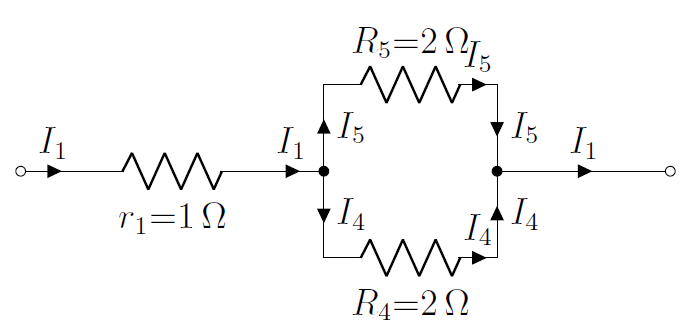
\includegraphics[width=0.5\linewidth]{files/bigcircuit_vals_r8-95d96b76bef1e0d43ff22f54d3083840.png}
\caption[]{The components of the effective $R_8$ resistor from Figure~\ref{fig:circuits:bigcircuit_vals_simp}. The current, $I_1$, coming from the battery goes through $r_1$ and then splits up.}
\label{fig:circuits:bigcircuit_vals_r8}
\end{figure}

The current $I_1$, that goes through the $\Delta V_1$ battery also goes through the $r_1$ internal resistance of the battery. That current then splits up into currents, $I_4$ and $I_5$, to go through the resistors $R_4$ and $R_5$. Although it should be obvious that half of $I_1$ will go through each resistor (since these are equal), we can determine this from applying Kirchhoff's rules to the combination of resistors in Figure~\ref{fig:circuits:bigcircuit_vals_r8}:
\begin{equation}
I_1&=I_4+I_5 \quad&\text{(junction)}\\
I_5R_5-I_4R_4&=0\quad&\text{(clockwise loop)}
\end{equation}
From the loop equation, we have:
\begin{equation}
I_5=\frac{R_4}{R_5}I_4=I_4
\end{equation}
since $R_4=R_5=2 {\rm \Omega}$. Since $I_4=I_5$, the junction equation gives:
\begin{equation}
I_5=\frac{1}{2}I_1=1.15 {\rm A}
\end{equation}
By solving for $I_4$ and $I_5$, we have now determined all of the currents through all of the segments of the original circuit in Figure~\ref{fig:circuits:bigcircuit_vals}.

\textbf{Discussion:} In this example, we showed how one can use a simplified circuit to solve the current through the effective resistors in the simplified circuit. Once those currents are known, we showed that it is straightforward to determine the currents through individual resistors that have been combined into effective resistors.
\end{framed}
\end{framed}

\begin{framed}
\textbf{Josh's Thoughts}\\
Solving a circuit can be daunting, especially if the diagram is drawn in an unfamiliar  way. While the circuits in this chapter are designed to be as easy to read as possible, many circuits are much more strange. For example, here is a circuit which you may come across:

\begin{figure}[!htbp]
\centering
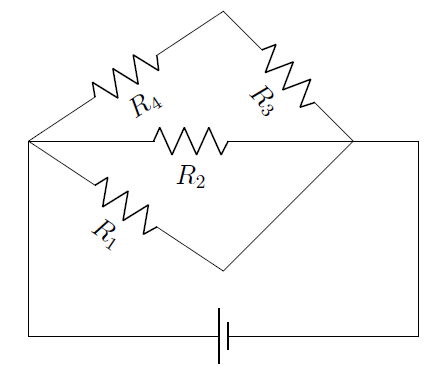
\includegraphics[width=0.4\linewidth]{files/circuit1Josh-7520d0c8826bca1fc6e734a164b2bfb1.png}
\caption[]{A weird looking circuit.}
\label{fig:circuits:circuit1Josh}
\end{figure}

The circuit in Figure~\ref{fig:circuits:circuit1Josh} May look like it is a difficult circuit to solve, but the diagram can be re-drawn to reveal the simplicity of the circuit:

\begin{figure}[!htbp]
\centering
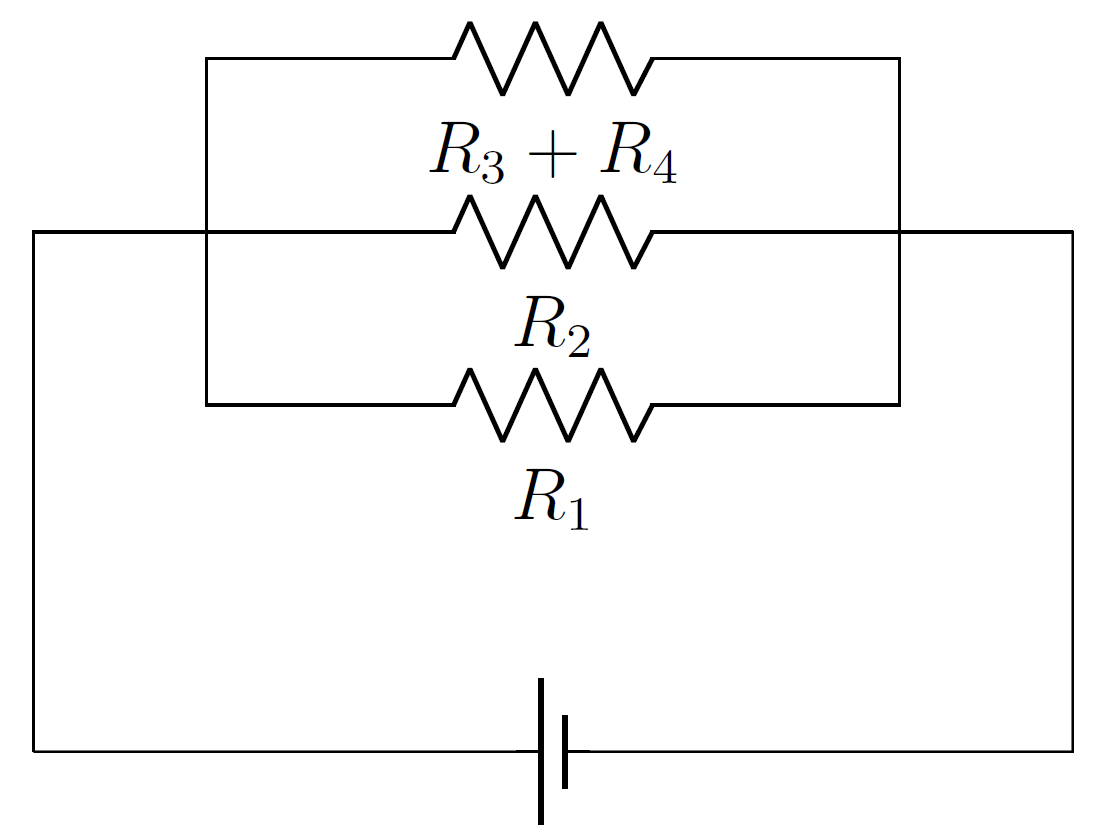
\includegraphics[width=0.4\linewidth]{files/circuit2Josh-4cb1604ed35f8db5448b4c644cbb8f91.png}
\caption[]{A much less weird looking circuit.}
\label{fig:circuits:circuit2Josh}
\end{figure}

What used to be a strange kite shape is now just a parallel circuit, which can be further simplified by calculating the effective resistance:
\begin{equation}
R_{eff} &= (R_1^{-1}+R_2^{-1}+(R_3+R_4)^{-1})^{-1}
\end{equation}
Which gives a series circuit with only one resistor:

\begin{figure}[!htbp]
\centering
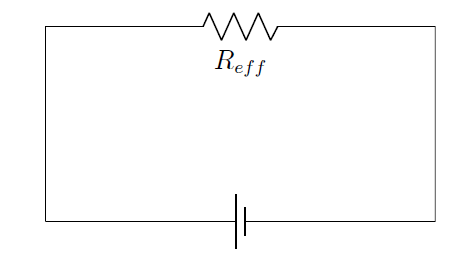
\includegraphics[width=0.4\linewidth]{files/circuit3Josh-a39cdccc8edb6d8a92b6f2e1d82a2f3a.png}
\caption[]{A simple circuit.}
\label{fig:circuits:circuit3Josh}
\end{figure}

Circuits can be drawn in many unique or potentially confusing ways, but knowing how to read the circuit and re-draw it can help make the diagram more legible and the circuit easier to solve.
\end{framed}

\subsubsection{Measuring current and voltage}

In this section, we describe how one can build devices to measure current and voltage. A device that measures current is called an ``ammeter'' and a device that measured voltage is called a ``voltmeter''. Nowadays, these are usually found within the same physical device (a ``multimeter''), which can also measure resistance (by measuring voltage and current, resistance can easily determined). We will limit our description to the design of simple analogue ammeters and voltmeters.

As we will see in Chapter {\textbackslash}ref\{chapter:magneticforce\}, it is straightforward to build a device that can measure very small amounts of current, by running the current through a coil in a magnetic field so that the coil can deflect a needle that indicates the amount of current. Such a device is called a ``galvanometer'' and is usually limited to measuring very small current (of order {\textbackslash}si\{mA\}). In this section, we describe how one can use a galvanometer in order to build both ammeters to measure large currents and voltmeters.

\paragraph{The ammeter}

An ammeter is built by placing a galvanometer in parallel with a ``shunt'' resistor, $R_s$. The shunt resistor is a small resistor that ``shunts'' (deflects) the current away from the galvanometer, so that most of the current goes through the shunt resistor. This is illustrated in Figure~\ref{fig:circuits:ammeter}, which shows the galvanometer (circle with the ${\rm G}$ inside), the internal resistance of the galvanometer, $R_G$, and the shunt resistor, $R_S$. The actual ammeter would be contained in a box and have two connectors (shown as ${\rm A}$ and ${\rm B}$ in the figure).

\begin{figure}[!htbp]
\centering
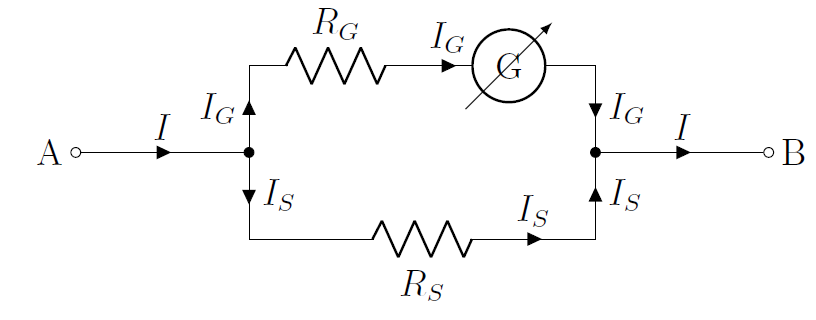
\includegraphics[width=0.55\linewidth]{files/ammeter-db19cc75fe976fb35097957e7bff97e2.png}
\caption[]{Constructing an ammeter from a galvanometer by placing a ``shunt'' resistor in parallel with the galvanometer.}
\label{fig:circuits:ammeter}
\end{figure}

By modelling the ammeter, we can determine the total current, $I$, that we would like to measure using the known values of the resistors and the current, $I_G$, measured by the galvanometer. Considering any of the two junctions, and a clockwise loop, we have:
\begin{equation}
I&=I_G+I_S \quad&\text{(junction)}\\
I_GR_G-I_SR_S&=0\quad&\text{(clockwise loop)}\\
\therefore I_S&=\frac{R_G}{R_S}I_G\\
\therefore I &= I_G+I_S=\left(1+\frac{R_G}{R_S}\right) I_G
\end{equation}
which allows us to determine the current $I$ from the current $I_G$, measured by the galvanometer. We also see that most of the current goes through the shunt (since $R_S$ is chosen to be smaller than $R_G$). The ammeter will have a total resistance, $R_A$, given by:
\begin{equation}
R_A=\frac{R_GR_S}{R_G+R_S}
\end{equation}
In order to measure the current through a specific segment of a circuit, an ammeter must be placed in series with that segment (so that the current that we want to measure will pass through the ammeter). Figure~\ref{fig:circuits:ammeterR} shows how to connect an ammeter (circle with the letter ${\rm A}$) in order to measure the current through a resistor, $R$.

\begin{figure}[!htbp]
\centering
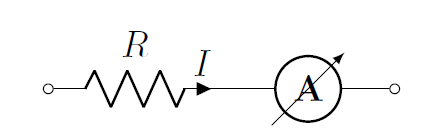
\includegraphics[width=0.4\linewidth]{files/ammeterR-6b1f56c0a866644a94700534fcf4da05.png}
\caption[]{An ammeter is placed in series with a resistor to measure the current through the resistor.}
\label{fig:circuits:ammeterR}
\end{figure}

\paragraph{The voltmeter}

A voltmeter is constructed by placing a large resistor, $R_V$, in series with a galvanomenter (that has internal resistance $R_G$), as illustrated in Figure~\ref{fig:circuits:voltmeter}. The voltmeter is designed to measure the potential difference between the terminals of the voltmeter (labelled ${\rm A}$ and ${\rm B}$ in the Figure).

\begin{figure}[!htbp]
\centering
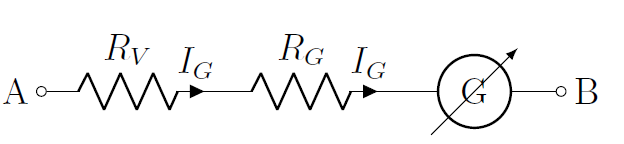
\includegraphics[width=0.5\linewidth]{files/voltmeter-49ef0913942c401600576df4ae715547.png}
\caption[]{Constructing an voltmeter from a galvanometer by placing a resistor in series with the galvanometer.}
\label{fig:circuits:voltmeter}
\end{figure}

Given the values of the resistors, and the current measured by the galvanometer, one can easily determine the potential difference between points ${\rm A}$ and ${\rm B}$, since the current measured by the galvanometer goes directly through each resistor:
\begin{equation}
\Delta V = V_B-V_A=-I_G(R_V+R_G)
\end{equation}
In order to measure a potential difference across a component, the voltmeter must be placed in parallel with the component. Figure~\ref{fig:circuits:voltmeterR} shows how to connect a voltmeter (circle with the letter ${\rm V}$) in order to measure the voltage across a resistor, $R$.

\begin{figure}[!htbp]
\centering
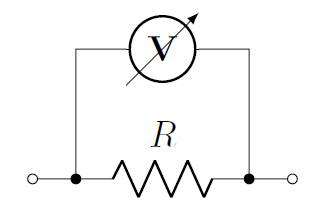
\includegraphics[width=0.3\linewidth]{files/voltmeterR-64b16d12078075d9e8cbf6f8dd3935e8.png}
\caption[]{A voltmeter is placed in parallel with a resistor to measure the voltage across the resistor.}
\label{fig:circuits:voltmeterR}
\end{figure}

When using an ammeter or a voltmeter, you will notice that these usually have buttons or dials to choose the range of currents or voltages to be measured. All the dial does is change the value of the shunt or series resistor in order to maintain a given maximum current through the galvanometer. An ohmmeter, to measure resistance, is simply an ammeter with a built-in fixed potential difference (so that by measuring current across a known potential difference, the resistance of the component can be determined).

\begin{framed}
\textbf{Example 19.4}\\
Two resistors with a resistance of $1 {\rm k\Omega}$ are placed in series with a $12 {\rm V}$ battery. A voltmeter with a total resistance of $R_V=10 {\rm k\Omega}$ is used to measure the voltage across one of the resistors. What reading does the voltmeter show?

\begin{framed}
\textbf{Solution}\\
Since the two resistors have the same resistance, and are in series with the battery, when no voltmeter is connected, the voltage across either resistor is easily shown to be $6 {\rm V}$. However, by connecting the voltmeter across one of the resistors, we modify the circuit, and we should expect the voltage that is read to be different than $6 {\rm V}$ (can you tell if it will be larger or smaller?). The circuit, with the voltmeter connected, is shown in Figure~\ref{fig:circuits:voltmeter2R}.

\begin{figure}[!htbp]
\centering
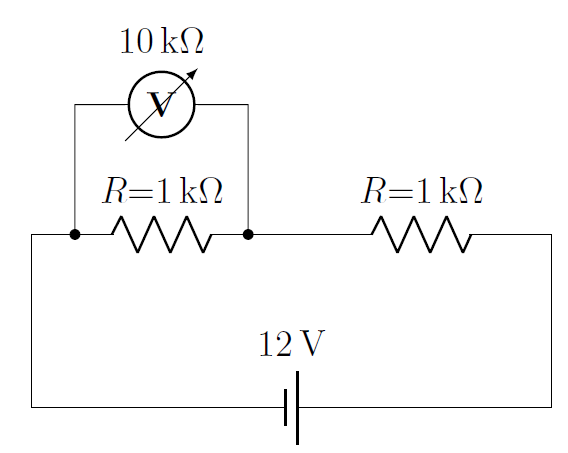
\includegraphics[width=0.35\linewidth]{files/voltmeter2R-b7592cd3b8ef50a3b49d46c3cf69f11e.png}
\caption[]{When using a voltmeter, the circuit is modified.}
\label{fig:circuits:voltmeter2R}
\end{figure}

We can model this circuit quite easily by combining the voltmeter (modelled as a resistor) in parallel with one of the resistors:
\begin{equation}
R_{eff}&=\frac{R_VR}{R_V+R}\\
&=\frac{(10 {\rm k\Omega})(1 {\rm k\Omega})}{(10 {\rm k\Omega})+(1 {\rm k\Omega})}\\
&=\frac{10}{11}{\rm k\Omega}=0.91 {\rm k\Omega}
\end{equation}
The sum of the voltage drops across the effective resistor and the other resistor must equal the potential difference across the battery (Kirchhoff's loop rule):
\begin{equation}
R_{eff}I+RI&=\Delta V\\
\therefore I &= \frac{\Delta V}{R_{eff}+R}=\frac{(12 {\rm V})}{(0.91 {\rm k\Omega})+(1 {\rm k\Omega})}=6.29e-3 {\rm A}
\end{equation}
The voltage drop across the effective resistor is the same as the reading on the voltmeter:
\begin{equation}
\Delta V_{voltmeter}=IR_{eff}=(6.29e-3 {\rm A})(0.91 {\rm k\Omega})=5.7 {\rm V}
\end{equation}
and the voltmeter reads a smaller voltage than there would be without the voltmeter.

\textbf{Discussion:} In this example, we saw that by using a voltmeter to measure a voltage in a circuit, we actually disturb the circuit. By placing the voltmeter in parallel with one resistor, we created an effective resistor with a resistance that is lower than the resistance of either the voltmeter or the resistor. This lowered the total resistance of the circuit, which increased the current. A larger current through the second resistor (without the voltmeter) leads to a larger voltage drop than $6 {\rm V}$ across that resistor. Thus, the voltage drop across the resistor with the voltmeter will be less than $6 {\rm V}$, as we found, since the two voltage drops need to add to $12 {\rm V}$. In general, when using a voltmeter, one needs a voltmeter with a very high resistance in order to minimize the disturbance to the circuit (if the voltmeter has a high resistance, only a small amount of current will be shunted from the resistor). In practice, voltmeters have resistance that are typically of the order of $1 {\rm M\Omega}$.
\end{framed}
\end{framed}

\subsubsection{Modelling circuits with capacitors}

{\textbackslash}begin\{review\}
* Section {\textbackslash}ref\{sec:potential:capacitors\} on capacitors.

{\textbackslash}end\{review\}
So far, we have modelled circuits where the current does not change with time. When a capacitor is included in a circuit, the current will change with time, as the capacitor charges or discharges. The circuit shown in Figure~\ref{fig:circuits:RCcircuit} shows an ideal battery{\textbackslash}footnote\{The model still holds for a real battery, since the internal resistance of the battery can just be included into the resistance of the resistor, $R$.\} ($\Delta V$), in series with a resistor ($R$), a capacitor ($C$, two vertical bars) and a switch (${\rm S}$) that is open.

\begin{figure}[!htbp]
\centering
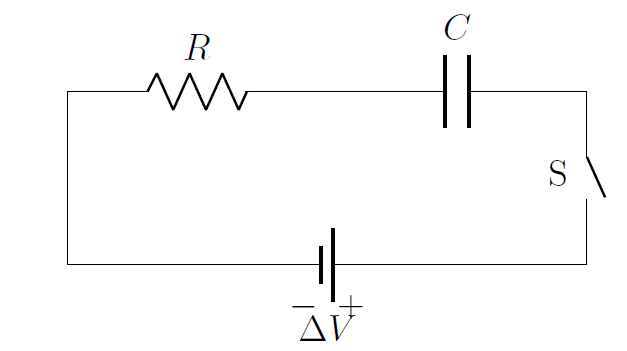
\includegraphics[width=0.4\linewidth]{files/RCcircuit-ed0f38181d5ef64b678a6171d86d88e5.png}
\caption[]{A simple circuit with a resistor, battery, and capacitor.}
\label{fig:circuits:RCcircuit}
\end{figure}

When the switch is open, current cannot flow through the circuit. If we assume that the capacitor has no charge on it, once we close the switch, current will start to flow and charges will accumulate on the capacitor. Electrons will leave the negative terminal of the battery, flow through the resistor and accumulate on the left side of the capacitor, which acquires a negative charge. This pushes electrons off of the right hand side of the capacitor, which then becomes positively charged. The electrons from the positive side of the capacitor then flow into the positive side of the battery, completing the circuit.

Eventually, the charges on the capacitor will build up to a point were they prevent any further flow of current. Once the left side of the capacitor is at the same potential as the left side of the battery, current will cease to flow. That is, eventually, the potential difference across the capacitor will be equal to that across the battery, and we can think of this as a circuit used to charge a capacitor. The current is high when the switch is first opened, but eventually goes down to zero as the capacitor charges. The current is thus time-dependent.

We can model this simple circuit (with the switch closed) using Kirchhoff's loop rule. The sum of the voltages across each component must sum to zero:
\begin{equation}
\Delta V - IR - \frac{Q}{C} = 0
\end{equation}
where we used the fact that the charge, $Q$, on a capacitor is related to the potential difference, $\Delta V_C$, across the capacitor by $Q=C\Delta V_C$. The current, $I$, is the rate at which charges flow through the circuit, and is thus equal to rate at which charges accumulate on the capacitor:
\begin{equation}
I=\frac{dQ}{dt}
\end{equation}
Substituting this into the loop equation, we obtain a separable differential equation for the charge on the capacitor as a function of time, $Q(t)$:
\begin{equation}
\Delta V - IR - \frac{Q}{C} &= 0\\
\Delta V - \frac{dQ}{dt}R - \frac{Q}{C} &= 0\\
\Delta V - \frac{Q}{C} &= \frac{dQ}{dt}R\\
C\Delta V - Q &= RC\frac{dQ}{dt}\\
\therefore \frac{dt}{RC}&=\frac{dQ}{C\Delta V - Q }
\end{equation}
This is similar to differential equations that we have solved previously (in fact, it is the same equation as in Example~6.4 where we looked at the effect of velocity-dependent drag). The solution to the equation, assuming that the switch is closed at $t=0$, is given by an exponential:
\begin{equation}
Q(t) = C\Delta V\left( 1 - e^{-\frac{t}{RC}} \right)
\end{equation}
Thus, the charge on the capacitor starts at zero when the switch is closed, and grows asymptotically until it reaches a value of $Q=C\Delta V$, which corresponds to the capacitor having the same potential difference across it as the battery. The value $\tau=RC$ is called the ``time constant'' of the RC circuit, and corresponds to the time at which the capacitor will reach about $(1 -e^{ -1})=63\%$ of its maximal charge. The current as a function of time is given by:
\begin{equation}
I(t)=\frac{dQ}{dt}=\frac{\Delta V}{R}e^{-\frac{t}{RC}}
\end{equation}
and we can see that at time $t=0$ the current is the same as if there were no capacitor present, and the current then decreases exponentially until it reaches zero.

\subsubsection{Summary}

Batteries are usually formed from a collection of electrochemical cells. Batteries provide a constant electric potential difference across their terminals, usually sustained by a chemical reaction, as long as the current through the battery is not too large (or the chemical reactions cannot be sustained).

An ideal battery has no resistance and can be modelled as a simple potential difference in a circuit. A real battery includes an internal resistance and be modelled in a circuit as an ideal battery in series with a resistor. The voltage across the terminals of a real battery is equal to the voltage across the terminals of the ideal battery only when no current flows through the internal resistance.

Circuits are modelled using circuit diagram that include components (such as batteries and resistors) and wires. Wires are always modelled as having no resistance, since their resistance can be included by placing the appropriate resistor along the wire. The electric potential is always constant along a wire with no resistance. When modelling a circuit, \textbf{one always models the direction of conventional current}; that is, current is always indicated as the direction in which positive charges flow (even if in reality, it is negative electrons that flow in the opposite direction).

Circuits should be thought of in terms of conservation of energy. Components produce a potential difference between sections of wire. Batteries correspond to an increase in potential (if going from the negative to the positive terminal), whereas resistors corresponds to a decrease in potential (if going in the same direction as current through the resistor).

Kirchhoff's rules allow us to model complex circuits. The junction rule states that: \textbf{The current entering a junction must be equal to the current exiting a junction.} This is a statement about conservation of charge. If charges are flowing into a junction, then the same amount of charges must flow back out of the junction per unit time.

The loop rule states that: \textbf{The net voltage drop across a loop must be zero.} This is a statement about conservation of energy indicating that as the potential energy of a positive charge increases as it goes through a battery, it will decrease by the same amount if it goes through a resistor that is connected to the terminals of that battery.

In order to \textbf{apply the loop rule}, we strongly suggest using the following procedure, after having made a clear, labelled diagram showing battery arrows and currents in the circuit:

\begin{enumerate}
\item Identify the loop, including starting position and direction.
\item Start at the beginning of the loop, and trace around the loop.
\item Each time a battery is encountered, \textbf{add the battery voltage if you are tracing the loop in the same direction as the corresponding battery arrow}, subtract the voltage otherwise.
\item Each time a resistor is encountered, \textbf{subtract the voltage across that resistor ($RI$, from Ohm's Law) if tracing the loop in the same direction as the current}, add the the voltage otherwise.
\item Once you have traced back to the starting point, the resulting sum must be zero.
\end{enumerate}

In general, we suggest the following procedure in order to use Kirchhoff's rules to model any circuit:

\begin{enumerate}
\item Make a good diagram of the circuit.
\item Simplify any resistors that can easily be combined into effective resistors (in series or in parallel).
\item Make a new diagram with the effective resistors, showing battery arrows, and labelling all of the nodes so that loops can easily be described.
\item Make a \textbf{guess} for the directions of the current in each segment.
\item Write the junction rule equations. Usually, you will get $M -1$ independent equations for $M$ loops.
\item Write the loop equations. Usually, you will get $M -1$ independent equations for $M$ loops.
\item This will lead to $N$ independent equations that one can solve for the $N$ different currents in the circuit.
\item Once you have determined all of the currents, if some of them are negative numbers, switch the direction of those currents in the diagram (they will be negative if you guessed the direction incorrectly).
\end{enumerate}

Current and voltage measuring devices (ammeters and voltmeters, respectively) can be constructed from a galvanometer, which measures small currents. An ammeter is constructed by placing a small shunt resistor in parallel with the galvanometer so that most of the current passes through the shunt resistor. The resulting ammeter must be placed in series with a component in order to measure the current through that component.

A voltmeter is constructed by placing a resistor in series with the galvanometer in order to reduce the current through the galvanometer. The resulting voltmeter must be placed in parallel with a component in a circuit in order to measure the voltage across that component. Note that because voltmeters and ammeters have a non-zero resistance, they will affect the circuit once they are connected.

When a capacitor is placed in a circuit, the current in the circuit will no longer be constant in time. If an uncharged capacitor with capacitance, $C$, is placed in a series circuit with a battery and a resistor of resistance, $R$, the capacitor will charge until the voltage across the capacitor is equal to that across the battery. Once the capacitor is charged, current ceases to flow in the circuit. The charges on a capacitor accumulate with a rate that decays exponentially; it will take an infinite amount of time for the capacitor to become fully charged. It will be charged to about 63\% of maximum charge after a period of time, $\tau=RC$, called the time constant of the capacitor.

\begin{framed}
\textbf{Important Equations}\\
\textbf{Ohm's Law:}
\begin{equation}
\Delta V &= IR
\end{equation}
\textbf{Junction Rule:}
\begin{equation}
\sum I_{in} &= \sum I_{out}
\end{equation}
\textbf{Loop Rule:}
\begin{equation}
\sum_{loop} \Delta V = 0
\end{equation}
\end{framed}

\subsubsection{Thinking about the material}

\begin{framed}
\textbf{Reflect and research}\\
\begin{itemize}
\item When did Galvani and Volta experiment with electric cells?
\item What is the largest voltage that Volta obtained with his voltaic pile?
\item How does one charge a rechargeable battery? What would the circuit look like?
\end{itemize}
\end{framed}

\begin{framed}
\textbf{To try at home}\\
\begin{itemize}
\item Research circuit diagrams of appliances you have at home.
\end{itemize}
\end{framed}

\begin{framed}
\textbf{To try in the lab}\\
\begin{itemize}
\item Propose an experiment to measure the change in current of an RC circuit as a capacitor builds up and releases charge.
\item Propose an experiment to determine the RC constant for a capacitor charging circuit.
\item Propose an experiment to measure the resistance of a voltmeter and compare your results with the manufacturer's.
\end{itemize}
\end{framed}

\subsubsection{Sample problems and solutions}

\paragraph{Problems}

\begin{framed}
\textbf{Problem 19.1}\\
A simple RC circuit as shown in Figure~\ref{fig:circuits:RCcircuit} contains a charged capacitor of unknown capacitance, $C$, in series with a resistor, $R=2 {\rm \Omega}$. When charged, the potential difference across the terminals of the capacitor is $9 {\rm V}$.

At time $t=0 {\rm s}$, the switch, ${\rm S}$, is closed, allowing the capacitor to discharge through the resistor. The current is then measured to be $I = 0.05 {\rm A}$ at $t = 5 {\rm s}$ after opening the switch.

\begin{itemize}
\item a. What is the capacitance of the capacitor?
\item b. What charge did the capacitor hold at $t = 2 {\rm s}$?
\end{itemize}

\begin{figure}[!htbp]
\centering
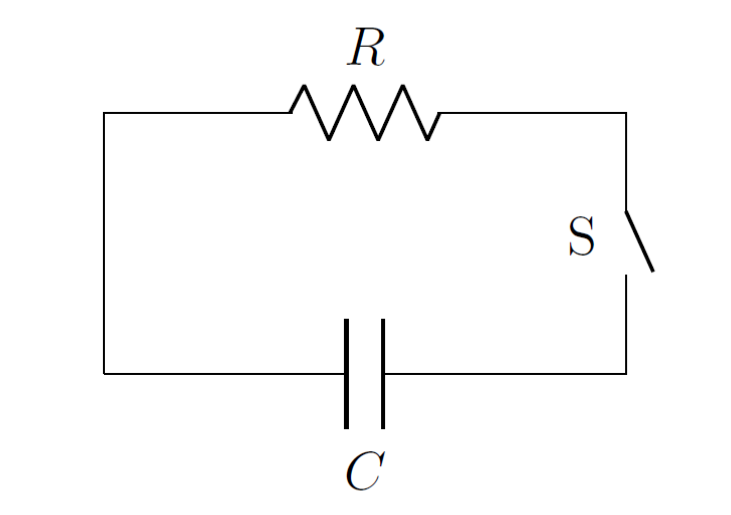
\includegraphics[width=0.3\linewidth]{files/RCcircuitCharge-10b05782ac2f5b4511023f1c0ed42294.png}
\caption[]{A simple circuit with a resistor and a capacitor.}
\label{fig:circuits:RCcircuitCharge}
\end{figure}
\end{framed}

\begin{framed}
\textbf{Problem 19.2}\\
A voltmeter with a resistance of $R_V = 20 {\rm k\Omega}$ is attached to a circuit with a battery of unknown voltage and two resistors with a resistance of $R = 2.5 {\rm k\Omega}$ as shown in Figure~\ref{fig:circuits:question2circuit}. The voltmeter reads that the voltage drop over one of the resistors is $\Delta V_{vm} = 5.647 {\rm V}$. What is the voltage drop, $V_R$, over each resistor when the voltmeter is removed from the circuit?

\begin{figure}[!htbp]
\centering
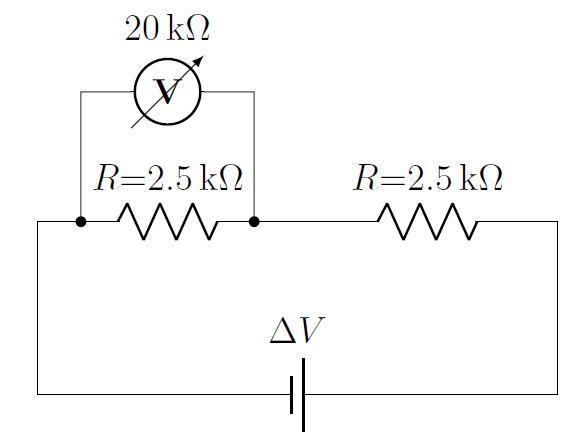
\includegraphics[width=0.45\linewidth]{files/question2circuit-ed8c1860995b2657c9e658d308b1eb62.png}
\caption[]{A circuit with a battery of unknown voltage.}
\label{fig:circuits:question2circuit}
\end{figure}
\end{framed}

\paragraph{Solutions}

\begin{framed}
\textbf{Solution 19.1}\\
\begin{itemize}
\item a. In this case, the capacitor is discharging as a function of time. At time $t=0$, the voltage across the capacitor is $\Delta V=9 {\rm V}$. We can model this discharging circuit in a similar way as we modelled the charging circuit.
\end{itemize}

We start with Kirchhoff's loop rule, which leads to a differential equation for the charge stored on the capacitor as function of time, $Q(t)$:
\begin{equation}
\Delta V - IR &=0\\
\frac{Q}{C} - IR &=0\\
\frac{Q}{C} - \frac{dQ}{dt}R &=0\\
\therefore \frac{dQ}{dt} = -\frac{1}{RC}Q
\end{equation}
This differential equation is straightforward to solve, since it says that the derivative of $Q(t)$ is equal to a constant multiplied by $Q(t)$. Thus, $Q(t)$ must be an exponential function:
\begin{equation}
Q(t) = Q_0 e^{-\frac{t}{RC}}
\end{equation}
where $Q_0$ is the (unknown) charge on the capacitor at $t=0$. You can easily verify that taking the derivative of this equation will result in the differential equation being satisfied.

Now that we have an equation for the charge as a function of time, it is straightforward to find the current, since it is just the time derivative of the charge. The current as a function of time, $I(t)$, is given by:
\begin{equation}
I &=\frac{dQ}{dt}=-\frac{1}{RC}Q=\frac{Q_0}{RC} e^{-\frac{t}{RC}}=I_0e^{-\frac{t}{RC}}
\end{equation}
where $I_0=\frac{Q_0}{RC}$ is the current at $t=0$.{\textbackslash}

We also know that the current through the resistor at $t=0$ is given by Ohm's Law, since, at that time, the voltage, $\frac{Q_0}{C}=9 {\rm V}$:
\begin{equation}
I_0=\frac{Q_0}{RC}=\frac{(9 {\rm V})}{(2 {\rm \Omega})}=4.5 {\rm A}
\end{equation}

We then know that the current, at time $t=5 {\rm s}$, is equal to $I(5)=0.05 {\rm A}$, allowing us to determine the capacitance:
\begin{equation}
I(5)&=I_0e^{-\frac{t}{RC}}\\
\ln\left( \frac{I(5)}{I_0} \right)&=-\frac{t}{RC}\\
\therefore C&=\frac{t}{R \ln\left( \frac{I_0}{I(5)} \right)}=\frac{(5 {\rm s})}{(2 {\rm \Omega})\ln\left( \frac{(4.5 {\rm A})}{(0.05 {\rm A})} \right)}=0.56 {\rm F}
\end{equation}

\begin{itemize}
\item b. To find the charge stored in the capacitor at $t = 2 {\rm s}$, we can use the function $Q(t)$ that we determined before:
\end{itemize}
\begin{equation}
Q(t=2 {\rm s})=Q_0 e^{-\frac{t}{RC}}
\end{equation}
where we can determine $Q_0$, now that we know the capacitance. $Q_0$ is the charge on the capacitor at time $t=0$, when the voltage across the capacitor is $9 {\rm V}$:
\begin{equation}
Q_0=C\Delta V = (0.56 {\rm F})(9 {\rm V})=5.0 {\rm C}
\end{equation}
At $t = 2 {\rm s}$, the charge on the capacitor is thus:
\begin{equation}
Q(t = 2 {\rm s})=(5.0 {\rm C})e^{-\frac{(2 {\rm s})}{(2 {\rm \Omega})(0.56 {\rm F})}}=0.84 {\rm C}
\end{equation}
\end{framed}

\begin{framed}
\textbf{Solution 19.2}\\
In order to know the voltage across one of the resistors, we need to determine the voltage that is across the battery. Once we have determined the voltage across the battery, the voltage across one of the resistors will just be half of that across the battery, since the two resistors have the same resistance.

We can model the circuit with the voltmeter in place, since we know the voltage across the parallel combination of the voltmeter and resistor (that voltage which is readout by the voltmeter). We can combine the voltmeter and one of the resistors into a an equivalent resistor, $R_{eff}$:
\begin{equation}
R_{eff} &= \frac{1}{R_V^{-1}+R^{-1}}\\
R_{eff} &= \frac{1}{(20 {\rm k\Omega})^{-1}+(2.5 {\rm k\Omega})^{-1}}\\
R_{eff} &= 2.22 {\rm k\Omega}\\
\end{equation}
Now that we have the effective resistance as well as the voltage drop across that effective resistor, we can solve for current through the circuit:
\begin{equation}
I &= \frac{\Delta V_{vm}}{R_{eff}}\\
I &= \frac{5.647 {\rm V}}{2.22 {\rm k\Omega}}\\
I &= 2.541 {\rm mA}\\
\end{equation}

Now that we have the current, we can combine the known resistances and determine the voltage drop across the battery.
\begin{equation}
\Delta V_{battery} &= I(R_{eff}+R)\\
\Delta V_{battery} &= (2.541 {\rm mA})(2.222 {\rm k\Omega}+2.5 {\rm k\Omega})\\
\Delta V_{battery} &= 12 {\rm V}\\
\end{equation}
Thus, with no voltmeter present, the voltage across each resistor is $6 {\rm V}$.
\end{framed}